\chapter{Auswertung}
    	\section{Germanium- und Siliziumdioden in Durchlassrichtung}
        	\begin{gnuplot}[terminal=pdf,terminaloptions={font ",10" linewidth 2},scale=1.2]
            		set fit errorvariables
					
                  	set xlabel "Spannung [V]"
                  	set ylabel "Stromstärke [mA]"
					set xrange [0:1]
                    set yrange [0:1]
                    
                    f(x) = a*exp(b*x)
                    g(x) = c*exp(d*x)
                    fit f(x) "Daten/A1a.txt" using 2:1 via a,b
                    fit g(x) "Daten/A1a.txt" using 3:1 via c,d
                    
                  	plot "Daten/A1a.txt" using 2:1 title "Germanium", "Daten/A1a.txt" using 3:1 title "Silizium", f(x), g(x)
			\end{gnuplot}
        \captionof{figure}[DurchlassGerSil]{Kennlinien der Dioden in Durchlassrichtung}
        Im Diagramm wurde die Fitfunktion 			
        \begin{equation}
        	f(x) = a \cdot \exp(b\cdot x)
        \end{equation}
        verwendet. \\
        
        Wenn wir davon ausgehen, dass Formel \ref{Sperrstrom-vereinfacht} gilt, können wir den Sperrstrom aus den gefitteten Werten ermitteln. \\
        
        Es ergibt sich:
	\begin{center}
		\begin{tabular}{c|cc}
			&  Germanium & Silizium\\ \hline
    		$I_s$ & $0.3\cdot 10^{-3} mA$ &  $0.04\cdot 10^{-6} mA$
		\end{tabular}
    \end{center}    
   		     
        
        \pagebreak
        
        \section{Germanium- und Silizium in Sperrrichtung}
        \begin{gnuplot}[terminal=pdf,terminaloptions={font ",10" linewidth 2},scale=1.2]
        	set xlabel "Spannung [V]"
			set ylabel "Stromstärke [Mikroampere]"
            
			f(x)=a*x+b
            g(x)=c*x+d
            
            set key left
            
            set xrange [-8:0]
            
            fit f(x) "Daten/A1c.txt" using 1:2 via a,b
            fit g(x) "Daten/A1c.txt" using 1:3 via c,d
           	
            plot "Daten/A1c.txt" using 1:2 title "Germanium", "Daten/A1c.txt" using 1:3 title "Silizium", f(x), g(x)
                    
			\end{gnuplot}
        \captionof{figure}[DurchlassGerSil]{Kennlinien der Dioden in Sperrrichtung}
        
       \ \\
       Die Werte passen nicht zu den im ersten Versuchsteil bestimmten Sperrströmen
        \pagebreak
        
        \section{Zenerdiode in Durchlass- und Sperrrichtung}
        	Trägt man Durchlass und Sperrrichtungskennlinien in einem gemeinsamen Diagramm auf erhält man die Z-Linie. \\
        	\begin{gnuplot}[terminal=pdf,terminaloptions={font ",10" linewidth 2},scale=1.2]
					
                  	set xlabel "Spannung [V]"
                  	set ylabel "Stromstärke [Mikroampere]"
                  	
                  	plot "Daten/A2a.txt" using 2:1 title "Durchlassrichtung", "Daten/A2b.txt" using 1:2 title "Sperrrichtung 
			\end{gnuplot}
        \captionof{figure}[DurchlassGerSil]{Gesamtkennlinie der Zener-Diode} 
        \ \\
        Hier spielt in der Sperrrichtung die spezielle Eigenschaft der Zener-Diode eine Rolle. Ab einer gewissen Sperrspannung nimmt ihr differentieller Widerstand exponentiell zu, während er vor dieser Spannung noch nicht vorhanden war.\ \\
        Bei einer Spannung von $ U = 5,75 V$ wurde mit der $\mu A$ -Skala ein Strom von $948 \mu A$ gemessen. Mit der mA-Skala wurde aber ein Strom von $960 \mu A$ gemessen. Die $\mu A$-Skala ist auf genaueres Messen ausgelegt, während die mA-Skala höhere Ströme aushält.
        
        \pagebreak
        
        \section{LEDs mit Oszilloskop}
        \begin{center}
        
         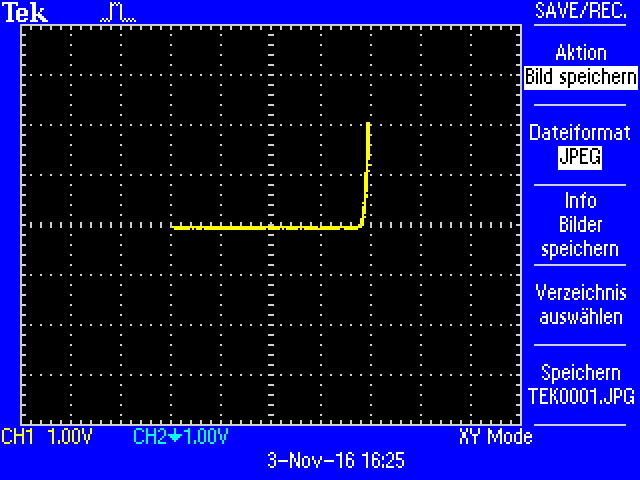
\includegraphics[scale=1]{Daten/TEK0001.JPG}
           \captionof{figure}[DurchlassGerSil]{Kennlinie der roten LED} 
         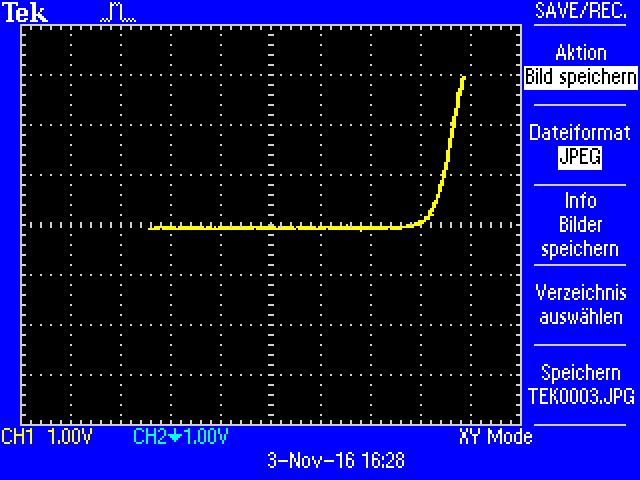
\includegraphics[scale=1]{Daten/TEK0003.JPG}
           \captionof{figure}[DurchlassGerSil]{Kennlinie der blauen LED} 
           \end{center}
        
       Die Schwellspannungen sind aus den Diagrammen abzulesen und sind:
       \begin{center}
       \begin{tabular}{c|c}
       &Schwellspannung\\ \hline
       Rot & $1,8 V$ \\
       Blau & $2,7 V$
       \end{tabular}
       \end{center}
       Damit lässt sich die Wellenlänge des Lichtes berechnen, das von der LED abgestrahlt wird.
       \begin{align*}
       		\lambda_{rot} & = \frac{h \cdot c}{e \cdot U_{rot}} \\
            & = \frac{6,626 \cdot 10^{-34} Js \cdot 0,3 \cdot 10^9 \frac{m}{s}}{1,6 \cdot 10^{-19} C \cdot 1,8 V} = 690,2 nm
       \end{align*} 
       \begin{align*}
       		\lambda_{blau} & = \frac{h \cdot c}{e \cdot U_{blau}} \\
            & = \frac{6,626 \cdot 10^{-34} Js \cdot 0,3 \cdot 10^9 \frac{m}{s}}{1,6 \cdot 10^{-19} C \cdot 2,7 V} = 460,1 nm
       \end{align*}
       
       Die errechneten Wellenlängen passen sehr gut zum Licht, dass von den LEDs abgestrahlt wird, wenn man für blaues Licht eine Wellenlänge von $420nm$ bis $490nm$ und $650nm$ bis $750nm$ für rotes Licht annimmt. \footnote{https://de.wikipedia.org/wiki/Licht}
	\pagebreak
